\documentclass{article}
\usepackage[utf8]{inputenc}
\usepackage[spanish]{babel}
\usepackage{graphicx}
\usepackage{amsmath}
\title{Modelos Matemáticos Discretos}
\author{JP}
\begin{document}
\maketitle
\section{Ecuaciones en diferencias}
\subsection{Primer orden}

Sabemos que $$\lim_{x\to\infty}\frac{1}{x}=0$$.

Calcular los valores propios de $A=
\begin{pmatrix}
1 & 2 \\
\pi & 4
\end{pmatrix}
.$ 

Consideremos e valor de una inversion de \$1000 que acumula interés de 1\% cada mes


EL valor de la inversión cuando han transcurrido $n$ meses es $$x_n=1000(1.01)^n$$
Una gráfica del resultado es 

\begin{center}
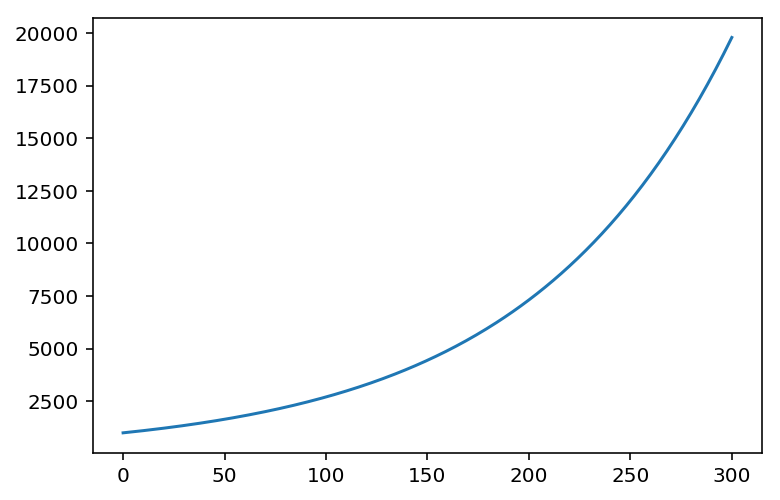
\includegraphics[width=8cm]{grafica}
\end{center}

Para encontrar este resultado, ocupamos que
$$\sum_{i=0}^{n-1}a^i=\frac{1-a^n}{1-a}$$

\begin{center}
\begin{tabular}{|c|r|}
\hline
0 & 1000 \\
1 & 1010\\
2 & 1021.21\\
\hline
\end{tabular}
\end{center}

\begin{center}
\huge
\textbf{NIÑOS NO HAGAN ESTO EN CASA}
\end{center}


\subsection{Segundo orden}

\end{document}
